Let $p$ be an odd prime. Arnaud has hung up $N\geq 1$ towels to dry on a washing line, each coloured either purple or yellow. Then, for each $1 \leq n \leq N$, he calculates what fraction of the first $n$ towels are yellow, and writes down these $N$ fractions in their irreducible form on a piece of paper. Julia finds the piece of paper the next day and notices that all of the fractions $\frac{1}{p}, \frac{2}{p}, \dots, \frac{p-1}{p}$ are on the paper. Prove that 
\[
N \geq \frac{p^3-p}{4}.
\]
\bigskip
\\
\textbf{Solution (Tanish):} Firstly, note that the only way to have a fraction with $p$ in the denominator is if the number of towels being counted is a multiple of $p$. Let $a_1, a_2, \dots, a_{p-1}$ denote the numerators of the fractions in the order they first appear in Arnaud's list, and $b_1, b_2, \dots, b_{p-1}$ the number of towels they correspond to. \\
Now observe that if we flip the colour of every single towel from purple to yellow and vice versa, then all the fractions will change from $\frac{a_i}{p}$ to $\frac{p-a_i}{p}$. Since all the fractions appear, this means that for every configuration of a given length, there is a configuration of the same length where the order of $1$ and $p-1$ are swapped in the list of the $a_i$, and so we can assume $1$ appears before $p-1$. \\
Suppose $p-1 = a_j$, and let $\lambda := \min(a_j, a_{j+1}, \dots, a_{p-1})$. We now make two case distinctions:
\begin{itemize}
    \item \textbf{$\lambda \ge \frac{p-1}{2}$.}\\
    In this case, let $a_k$ be the last of the numerators $1, 2, \dots, \lambda-1$ to appear in the list; it is clear that $k \ge \lambda-1$. Furthermore, note that this means at least $p(\lambda-1)$ towels are being taken into consideration (each new fraction needs at least $p$ towels between it and the previous fraction) and so $b_k \ge p \cdot (\lambda-1)$. The number of purple towels up to this point is therefore at least $\frac{p-a_k}{p} \cdot p \cdot (\lambda-1) = (p-a_k) \cdot (\lambda-1) \ge \frac{p+1}{2} \cdot \frac{p-1}{2} = \frac{p^2-1}{4}$. It follows that since $a_j  = p-1$ appears after this point, the purple towels by that point must only be $\frac{1}{p}$ of $b_j$ but there will be at least $\frac{p^2-1}{4}$ of them, so $\frac{p^3-p}{4} \le b_j \le N$ as desired. 
    \item \textbf{$\lambda < \frac{p-1}{2}$.}\\
    Define $a_k$ as in the previous case, and note that we still have at least $(p-a_k) \cdot (\lambda-1)$ purple towels in the first $b_k$ towels. This implies that $b_j$ is at least $p \cdot (p-a_k) \cdot (\lambda-1)$; so we have at least $(p-1) \cdot (p-a_k) \cdot (\lambda-1)$ yellow towels in the first $b_k$ towels. Now let $\lambda = a_l$; we see that since $a_l$ comes after $b_j$, the yellow towels must only be $\frac{\lambda}{p}$ of $b_l$ but there will be at least $(p-1) \cdot (p-a_k) \cdot (\lambda-1)$ of them, so $N \ge b_l \ge \frac{p \cdot (p-1) \cdot (p-a_k) \cdot (\lambda-1)}{\lambda} \ge p \cdot (p-1) \cdot \frac{p+1}{2} \cdot \frac{1}{2} = \frac{p^3-p}{4}$ as desired. \\
    \bigskip
\end{itemize}    
\emph{Remark:} The intuition behind this line of thinking is as follows: first, you test the case where $a_i = i$ and you notice the symmetry by testing the case $a_i = p-i$, allowing you to make the WLOG statement. Whilst observing these two cases, you notice the "issue" appears to be around the middle of the $a_i$ as it is by this point that too many purple towels have accumulated: even if you only have yellow towels from that point on, you will need too many before their total proportion is $\frac{p-1}{p}$. This encourages you to immediately conclude in the case where there are too many "small fractions" before $\frac{p-1}{p}$ and so now the question is what happens in the other case, where there are many large fractions at the start? In this case, the issue will become the large number of purple towels you have to add after $\frac{p-1}{p}$ in order to reduce the proportion to that of the smallest fraction that appears afterwards, and so you work with this instead. This problem is a nice exercise in formalising observations like this mathematically. 

\bigskip

\textbf{Marking Scheme (additive):}\\
Here, the use of the word "fraction" implies a fraction with denominator $p$. \\
If students reformulate the problem (for example, algebraically) they will not receive points for having changed the problem statement, but any progress made in alternative formulations will receive the equivalent points from the combinatorial version. 
\begin{itemize}
%\item 0P: Noting that the total number of towels when Arnaud wrote down one of the fractions must be a multiple of $p$.
\item 1P: Any evidence that the student has calculated $N \ge \frac{p^3-p}{4}$ in the case where the fractions appear in either ascending or descending order \emph{or} introducing the two inequalities $a_ib_i < a_{i+1}b_{i+1}$, $a_{i+1}b_{i+1} - a_ib_i \le (b_{i+1}-b_i)p$
%\item 0P: Noticing the symmetry when swapping purple and yellow towels.
%\item 0P: Using said symmetry to say "WLOG $\frac{1}{p}$ appears before $\frac{p-1}{p}$..." or vice versa.
\item 1P: Placing one of the two extremal fractions somewhere in the list \emph{and} considering either the maximum or minimum of the sets of fractions either before or after it. 
\item 1P: Noting that (for any particular $k$) at least one of the fractions $\frac{1}{p}, \dots, \frac{k}{p}$ will appear after at least $kp$ towels have been counted in total, or a symmetric observation based on whether the student is counting from first fraction to last or last to first, and if their extremal value is $1$ or $p-1$
\item 1P: Considering the first $\frac{p+1}{2}$ fractions.
\item 1P: Solving the case where all the fractions $\frac{1}{p}, \dots, \frac{p-1}{2p}$ appear before $\frac{p-1}{p}$.
\item 2P: Solving the case where some fraction $\in \{ \frac{1}{p}, \dots, \frac{p-1}{2p} \}$ appears after $\frac{p-1}{p}$. 
\end{itemize}
Students do not need to justify why $N$ is an integer value. 

\begin{center}
   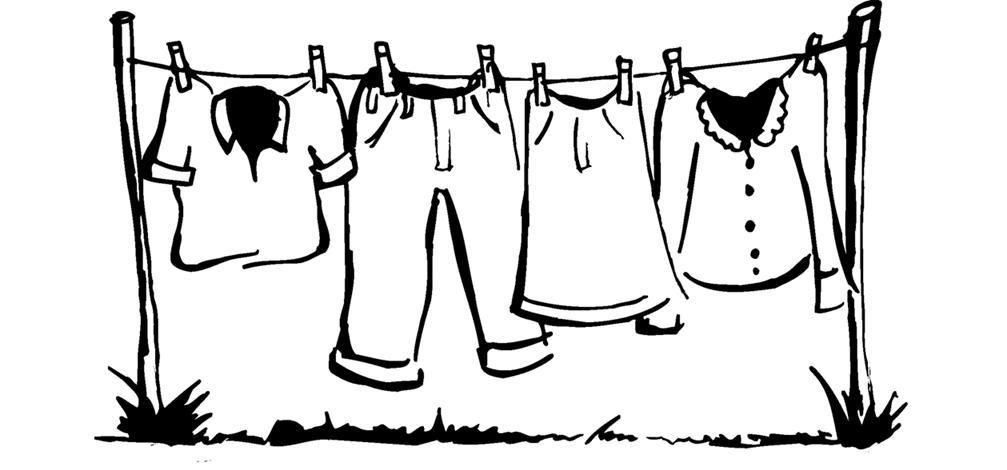
\includegraphics[scale=1]{2021/Selektion/muesterlosung/solutions/towel.png}
\end{center}

The following observations are not worth any points: 
\begin{itemize}
    \item Noting that the total number of towels when Arnaud wrote down one of the fractions must be a multiple of $p$.
    \item Noticing the symmetry when swapping purple and yellow towels.
    \item Using said symmetry to say "WLOG $\frac{1}{p}$ appears before $\frac{p-1}{p}$..." or vice versa.
\end{itemize}